\section{Data}
\label{sec:data}

One critical step is to inspect the reliability of the data set before using the data for analysis. The data set is a subsample of the \ac{CPS}. The \acs{CPS}, sponsored jointly by the U.S. Census Bureau and the U.S. Bureau of Labor Statistics, is the primary source of labor force statistics for the population of the United States. The \acs{CPS} is one of the oldest, largest, and most well-recognized surveys in the United States \cite{ipums_2020}. We also examined the statistical sampling techniques and designs of \acs{CPS}. Therefore, it is reasonable to believe the data set will provide reliable information.

We eliminate \textit{Year} and \textit{Month} in our data to reduce the complexity of working with panel data. Outliers are also narrowed out after drawing the Box-and-Whisker plots in Stata to preserve integrity. After that, we obtain summary statistics (see Table \ref{tab:summary_statistics}) and scatterplots of the ordinal variables in matrix form (see Figure \ref{fig:matrix}). Our data set contains a variety of people whose annual ages are mostly in range 14000 to 78000, aging from 21 to 63 with education level from 5th-grade to doctoral, given the means and the standard deviations. Whether people are male, nonmarried, or born in the US are included for our economic interests as well. 

\begin{table}
\scriptsize
\begin{adjustbox}{width=\textwidth}
\begin{tabular}{l*{1}{ccccc}}

\hline\hline

Variables\footnotemark   & Observation&        Mean&Standard Deviation&         Min&         Max\\
\hline
Wage        &       71800&    45570.07&       26987.01&        6740&  120000\\
Age         &       71800&       42.31&          13.92&          15&       85\\
Education   &       71800&       89.52&          22.17&          20&      125\\
Male        &       71800&        0.51&           0.50&           0&        1\\
Nonmarried  &       71800&        0.30&           0.45&           0&        1\\
US          &       71800&        0.81&           0.39&           0&       1\\
\hline\hline

\end{tabular}
\end{adjustbox}
\caption{\label{tab:summary_statistics}
Summary statistics for the research variables.}
\end{table}

\footnotetext{\textit{Wage} and \textit{Education} are ordinal variables. The higher the number, the higher the salary or degree.}
\footnotetext{\textit{Male}, \textit{Nonmarried} and \textit{US} are indicator variables. See the Code Book for specifics in Reference \cite{ipums_2020}.}


\begin{figure}[htp]
  \centering
  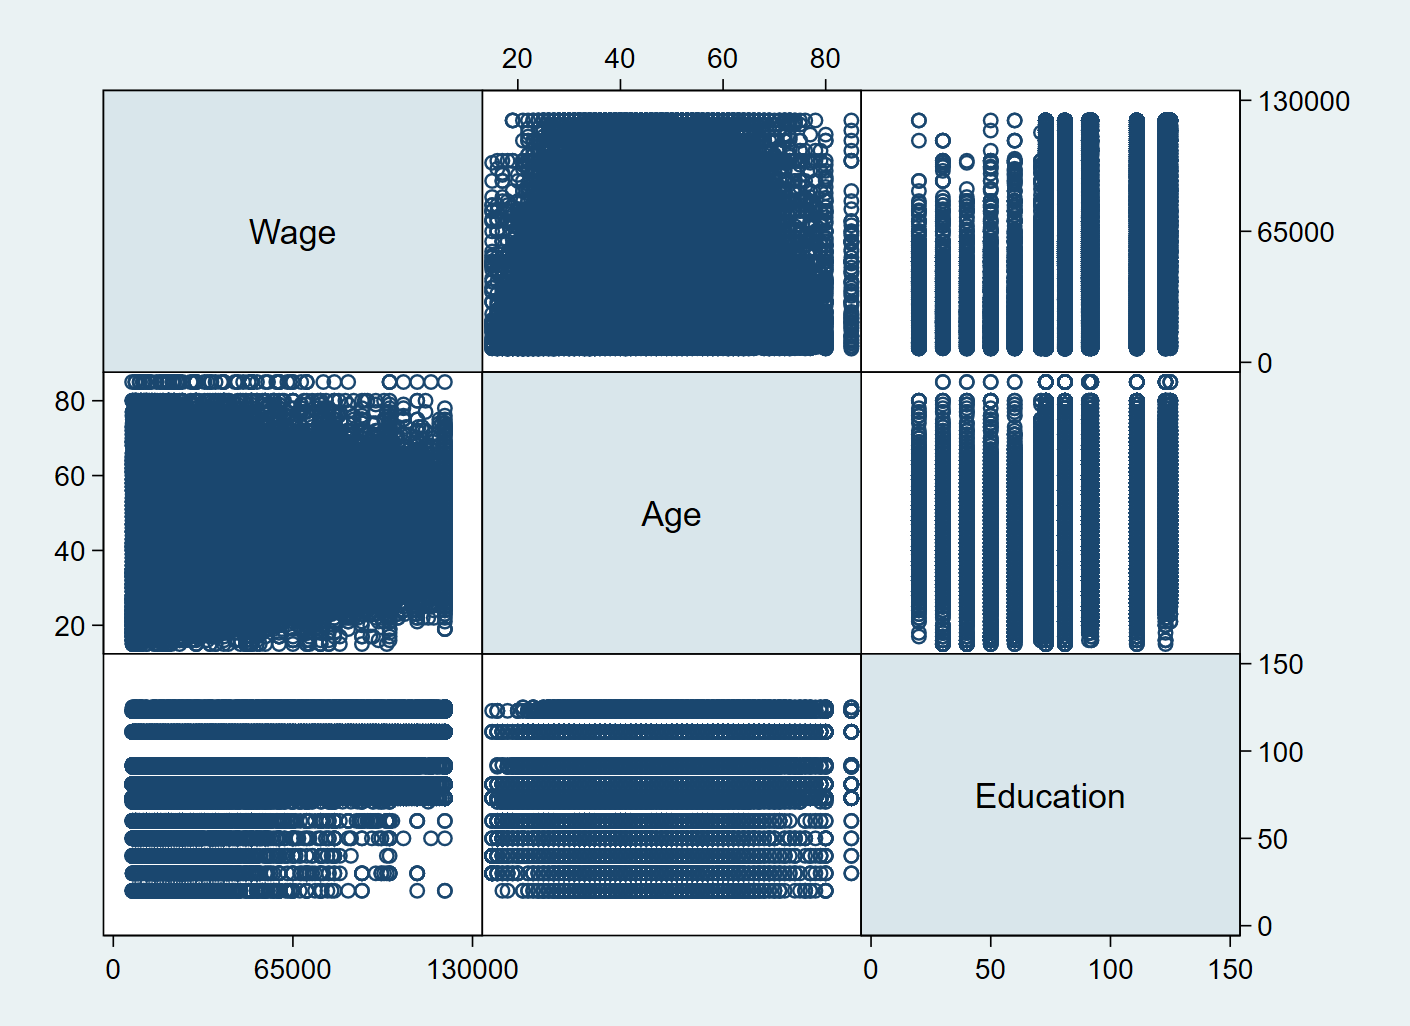
\includegraphics[scale=0.2]{{figures/graph_matrix}}
  \caption{\label{fig:matrix}
  \textit{graph matrix}\protect\footnotemark of approximately continous regression variables
   }
\end{figure}

\footnotetext{\textit{graph matrix} is a Stata command used to draw a scatterplot matrix to illustrate the bivariate relationships.}

\noindent We came up with the following observations from the summary statistics and the figure:
\begin{enumerate}
\item \textit{Wage} contains large integer dollar values. According to rules of thumb, it is more appropriate and natural to use logarithms\footnote{We use natural logarithm $\ln$ for simplicity throughout the paper.} to model \textit{Wage} as labor economists do \cite{stock_watson_2019, wooldridge_2020}.

\item We observe an implicit quadratic relationship between \textit{Wage} and \textit{Age}, though the width between the zeros of the parabola is large, which hides the potential relationship. Likewise, using a linear or an exponential function to describe \textit{Wage} and \textit{Education} is suitable \cite{wooldridge_2020}. To improve the likelihood of getting the most accurate model, we reviewed previous economic literature and concluded that our conjecture on the model would output more satisfactory goodness of fit.

\item For binary variables \textit{Male}, \textit{Nonmarried} and \textit{US}, the original form without any modification is good enough, but some interacted terms for the independent variables are needed for fitness. Based on past literature, we include \textit{Age}$\times$\textit{Education}, \textit{Education}$\times$\textit{Male} and so forth for exploration. Thus, we predict a positive linear relationship between \textit{Wage} and \textit{Male}, \textit{US}, and the opposite for \textit{Nonmarried}.
\end{enumerate}

After that, we run regressions and test which model is best given current data. However, there are some constraints regarding the data set. First, compared to time series data or panel data, cross-sectional data provide difficulty to justify if the cause and effect relationship follows exposure in time or exposure results from that effect. Moreover, the chronological ordering of the observations may provide essential information in time series data \cite{wooldridge_2020}. In this empirical analysis, cross-sectional data fulfill our goals.